We develop an approach to designing a reconfigurable manufacturing
system in which a swarm of homogeneous robots assembles static parts
into different types of products.  The system must respond quickly
to produce desired amounts of products, which can change at discrete
points in time, from any initial set of parts.  Since it is
difficult, if not impossible, to efficiently control a large robot
population through centralized algorithms, we employ a decentralized
strategy in which robots operate autonomously and use local
communication. The strategy can be readily implemented on
resource-constrained robots, and it is scalable in the number of
robots and parts and robust to changes in robot population.

The robots move randomly within a closed arena, encountering parts
and other robots at probability rates that are determined by the
physical parameters of the system and by sensor and environmental
noise.  We model this behavior using a realistic 3D physics
simulation, which we refer to as a {\it micro-continuous model}
since it encompasses the continuous dynamics of individual robots.
 The system can be approximated as well-mixed, and the robot-part and
robot-robot interactions are analogous to chemical reactions between
molecules.  Hence, like a set of chemical reactions, our system can
be represented by the Stochastic Master Equation
\cite{ref:Gillespie76}.  Various methods exist to numerically
simulate the evolution of a system governed by this model
\cite{Gillespie:2007p1788,Puchalka:2004p4312}.  We call this the
{\it complete macro-discrete model} because it describes a
continuous-time Markov process whose states are the discrete numbers
of system components.  When there are large numbers of parts, the
system can be abstracted to an ordinary differential equation (ODE)
model, which we call a {\it macro-continuous model} since its state
variables are continuous amounts of the parts.

Our work is similar in objective to studies on programmable
self-assembly for modular robots~\cite{Bishop:2005p2706,
Klavins:2007p2600, McNew:2008p2781, Klavins:2008p3969}.  The system
in this work is a set of homogeneous triangular robots that move
around randomly on an air table and assemble into
 components according to a plan that is constructed using
{\it graph grammars}, which are rules that define interactions
 between robots.  Graph grammars can be constructed
automatically to produce a given predefined
assembly~\cite{Klavins:2008p3969}.  The probabilities of a newly
formed component to detach into different combinations of parts can
be optimized to maximize the number of a desired assembly at
equilibrium \cite{Klavins:2007p2600}.  However, this optimization
requires the enumeration of all system states reachable from the
initial state.

%In addition, the assembly plan relies on kinetic rate constants that
%must be measured from simulations.

%But the main difference is that we build our optimization and whole
%approach directly with the rates thought as a basic feature. Klavins
%adds them later, modifying the plan he already optimized before.

Our approach to assembly system design allows for improved
scalability and flexibility. We consider a scenario in which a
heterogeneous set of parts is assembled into two types of final
products.  To provide theoretical guarantees on performance, we
employ the ``top-down" design methodology presented in
\cite{Berman:2006p10108, bib:berman2, Halasz:2007p10106} for
reallocating a swarm of robots among a set of sites/tasks in a
desired distribution.  This methodology was applied to a linear
model; here we extend it to a nonlinear (specifically, multi-affine)
model with robot interactions.  We construct this {\it complete
macro-continuous model} of the system using the Chemical Reaction
Network (CRN) framework
\cite{Feinberg:1979p10907,JamesWilkinson:2006p10341}, which has been
studied extensively for theoretical insight into biochemical
systems. We compute reaction rate constants in the model from
physical properties of the robots and environment and check that the
model accurately predicts the results of the micro-continuous model.
Then we simplify this abstraction to a {\it reduced macro-continuous
model} with the same rates and use the model to optimize these rates
for fast convergence to a target distribution of products, using an
approach similar to \cite{bib:BermanCDC08, ref:BermanTRO08}. The
optimization problem is independent of the number of parts and
scales only with the number of rates.  We simulate the reduced model
with optimized rates for different target distributions, map the
rates onto probabilities of assembly and disassembly which are used
as control policies in the micro-continuous model, and observe this
system's convergence behavior.

Fig. \ref{fig:fourlevel} illustrates the relationships among the
four levels of system abstraction discussed and the methods we use
for designing the system and analyzing its behavior.

\begin{figure}[t]
\centering
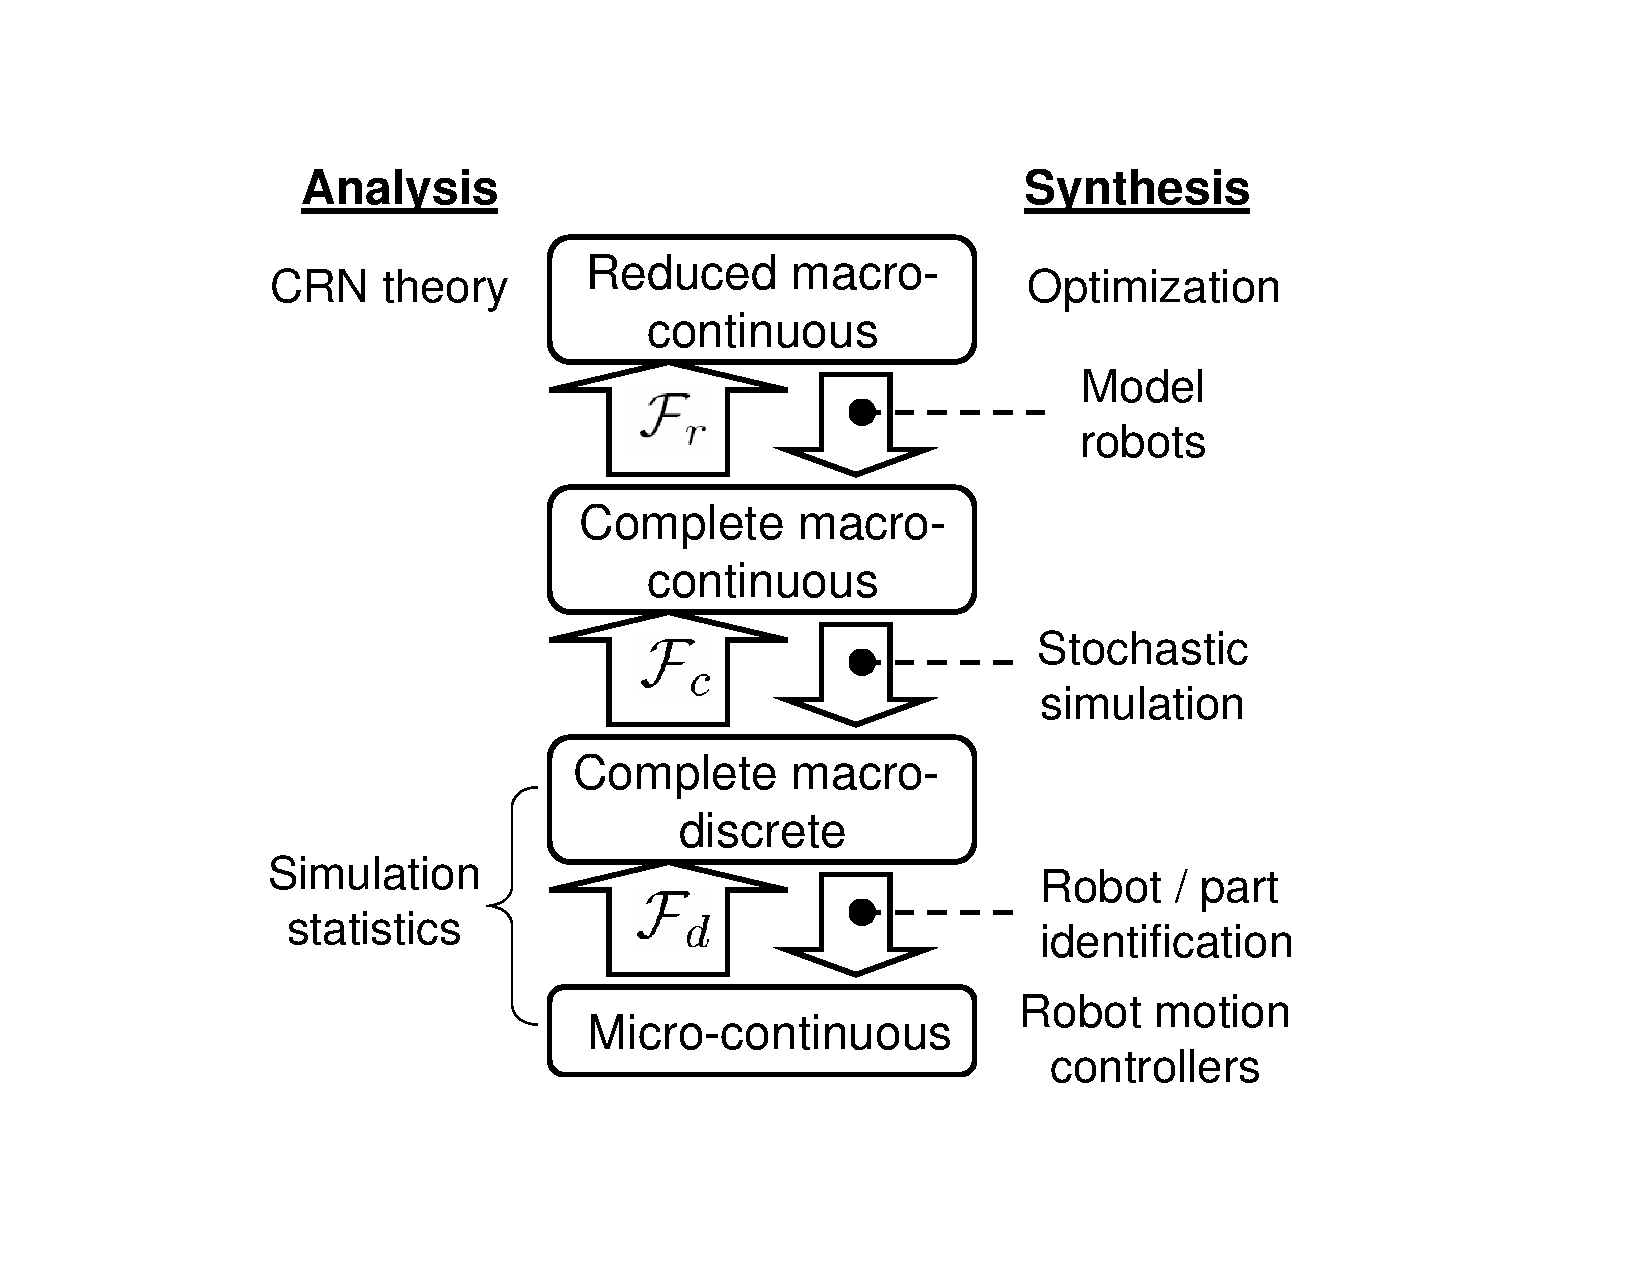
\includegraphics[trim= 30mm 30mm 30mm 20mm, clip,scale=0.35,angle=0]{img/FourLevels2.pdf}
\caption{Levels of abstraction of the assembly system with analysis
and synthesis methodologies.  The high-dimensional micro-continuous
model is mapped to lower-dimensional representations, the
macro-discrete and macro-continuous models, through the abstractions
$\mathcal{F}_d$ and $\mathcal{F}_c$ using the theoretical
justification in \cite{Gillespie:2007p1788}.  Under certain
assumptions (see Section \ref{sub:simple_macro_continuous_model}),
the complete macro-continuous model can be mapped to a
lower-dimensional model via the abstraction $\mathcal{F}_r$.}
\label{fig:fourlevel}
\end{figure}

%The desired ratio of final products is achieved, although some
%tuning of the [WHICH?] model is needed to reduce discrepancies with
%the physical system.

%[WILL PUT 3-LEVEL FIGURE HERE (?)]

%optimize the rate constants in a {\it reduced macro-continuous
%model}

%This optimization is mapped back onto the macro and the micro
%discrete, realizing a top-down control of the system.

%In this approach, the particularities of the assembling process, such as geometric
%difficulties and disassemblies due to shocks, are not taken into account.

% stochastic model has a more legitimate physical basis?

% Modular robotics encompass any robotic system that can deliberately change
       % its own shape, in order to adapt to new circumstances, perform new tasks or recover
       % from damage~\cite{Shen:2007p2613}.

%A graph grammar is a set of rules transforming a graph when
       % applied on it.

%The assembly process is modeled as a sequence of rules that
%transform the initial set of parts into a final graph that
%represents the final assembly.

%Upon collision, the parts use the graph grammar

%These grammars are then used with the robots to converge to a final
%shape constructed only by self-assembly.

% more generality in the components.

%This is also why we will use an approach using Chemical Reaction
%Networks for our plans
%         and models: they are build to take into account the intrinsic reaction rates of the
%         systems.

%to construct efficient simulations and provide

%Webots is based on ODE, an open source physics engine for simulating
%3D rigid body dynamics. Such a simulator allows us to performs
%systematic experiments faster than real-time and with null
%fabrication costs.

%a predefined distribution of components
